\documentclass[12pt]{article} % use larger type; default would be 10pt
\usepackage[utf8]{inputenc} % set input encoding (not needed with XeLaTeX)

\setlength{\parindent}{0in}
\setlength{\parskip}{0.2in}

\usepackage{geometry} % to change the page dimensions
\geometry{a4paper} %
\geometry{top=0.5in}
\usepackage{graphicx,color} % support the \includegraphics command and options
%primary color palette

%%% PACKAGES
\usepackage{amsmath}
\usepackage{amsthm}
\usepackage{amsfonts}
\usepackage{booktabs} % for much better looking tables
%\usepackage[]{fullpage} 
\usepackage{array} % for better arrays (eg matrices) in maths
\usepackage{paralist} % very flexible & customisable lists (eg. enumerate/itemize, etc.)
\usepackage{verbatim} % adds environment for commenting out blocks of text & for better verbatim
\usepackage{subfig} % make it possible to include more than one captioned figure/table in a single float
\usepackage{multirow} 
\usepackage{rotating}
\usepackage{amsthm}
\usepackage{caption}
\usepackage{tcolorbox}

\theoremstyle{definition}
\newtheorem{definition}{Definition}[section]

\theoremstyle{theorem}
\newtheorem{theorem}{Theorem}[section]

\AddToHook{cmd/section/before}{\clearpage}

\title{The Euler Spiral: Speaking Notes}
\author{Max Mussavian}

\begin{document}
	\date{16th May 2022}
    \maketitle
\section{Outline}
\begin{tcolorbox}
	\begin{itemize}
		\item Definitions and Derivations: parametric curves, lengths and curvature
		\item Relating curvature to the curve length
		\item Calculating arc length integrals
		\item Plotting the Euler spiral and other fun curves
		\item Application: designing railways and roads
	\end{itemize}
\end{tcolorbox}
Today I'm going to talk about a very special curve that was discovered by James Bernoulli and Leonhard Euler 300 years ago. That is a curve that gets more “curved” the “longer” the curve gets [use air quotes when saying curved and longer]. 
These curves are quite common around us from cantilever bridges, roads, railways to rat’s whiskers and the way that Formula One drivers drive around a racetrack. In order to derive these curves Euler and subsequent mathematicians had to come up with the definition of curves, length of curves and curvature. Which led to the field of differential geometry -- another first for Euler.
So my talk today is going to be about
\begin{itemize}
\item	the definitions and derivation of curves in $\mathbb{R}^2$, arc length and curvature.
\item Then I'm going to show you how you can relate curve length and curvature to define arbitrary curves.
\item In the simplest case we're going to look at curves where curvature is proportional to curve length. This was the original curve derived by Euler. This will require us to solve a pair of integrals which should now called Fresnel integrals.
\item I'm going to show you what type of curves you can construct by looking at some more general functions of curvature in terms of curve length.
\item Finally I'm going to show you that thanks to Euler are you don't get sick every time you turn off the motorway or take a train.
\end{itemize}

\section{Parametric curves}
\begin{tcolorbox}
	All curves in this talk are in $\mathbb{R}^2$.
	\begin{definition}[Parametric curve]
		A parametric curve is a smooth function that is defined on an open interval $(a, b)$ and takes values in $\mathbb{R}^2$ of the form $(x(t), y(t))$.
		\newline
		The set of points traced out by the curve is called the \textbf{trace}.
	\end{definition}
\end{tcolorbox}

We're going to start off with the definition of a curve. 

The curves we’re going to be working with takes values in $\mathbb{R}^2$.
 
The curves are functions that are defined in terms of a parameter $t$. $t$ which takes values in an open interval which could be infinite.

You can think of $t$ as time as this point but it doesn’t have to be -- as we will see later. 

This is different to the way you may seen curves before such as $x^2 + y^2 = 1$ which are called non-parametric cures. For our talk it turn out that parametric curves are much easier to work with.

The curves then give us the coordinates in the Cartesian plane and the coordinates the curve takes are called the trace.

Finally we require the curves to be smooth - that means they are continuous and differentiable as we will see later. 


\section{Length of a curve segment}
\begin{tcolorbox}
	\begin{minipage}{\linewidth}
		\centering
		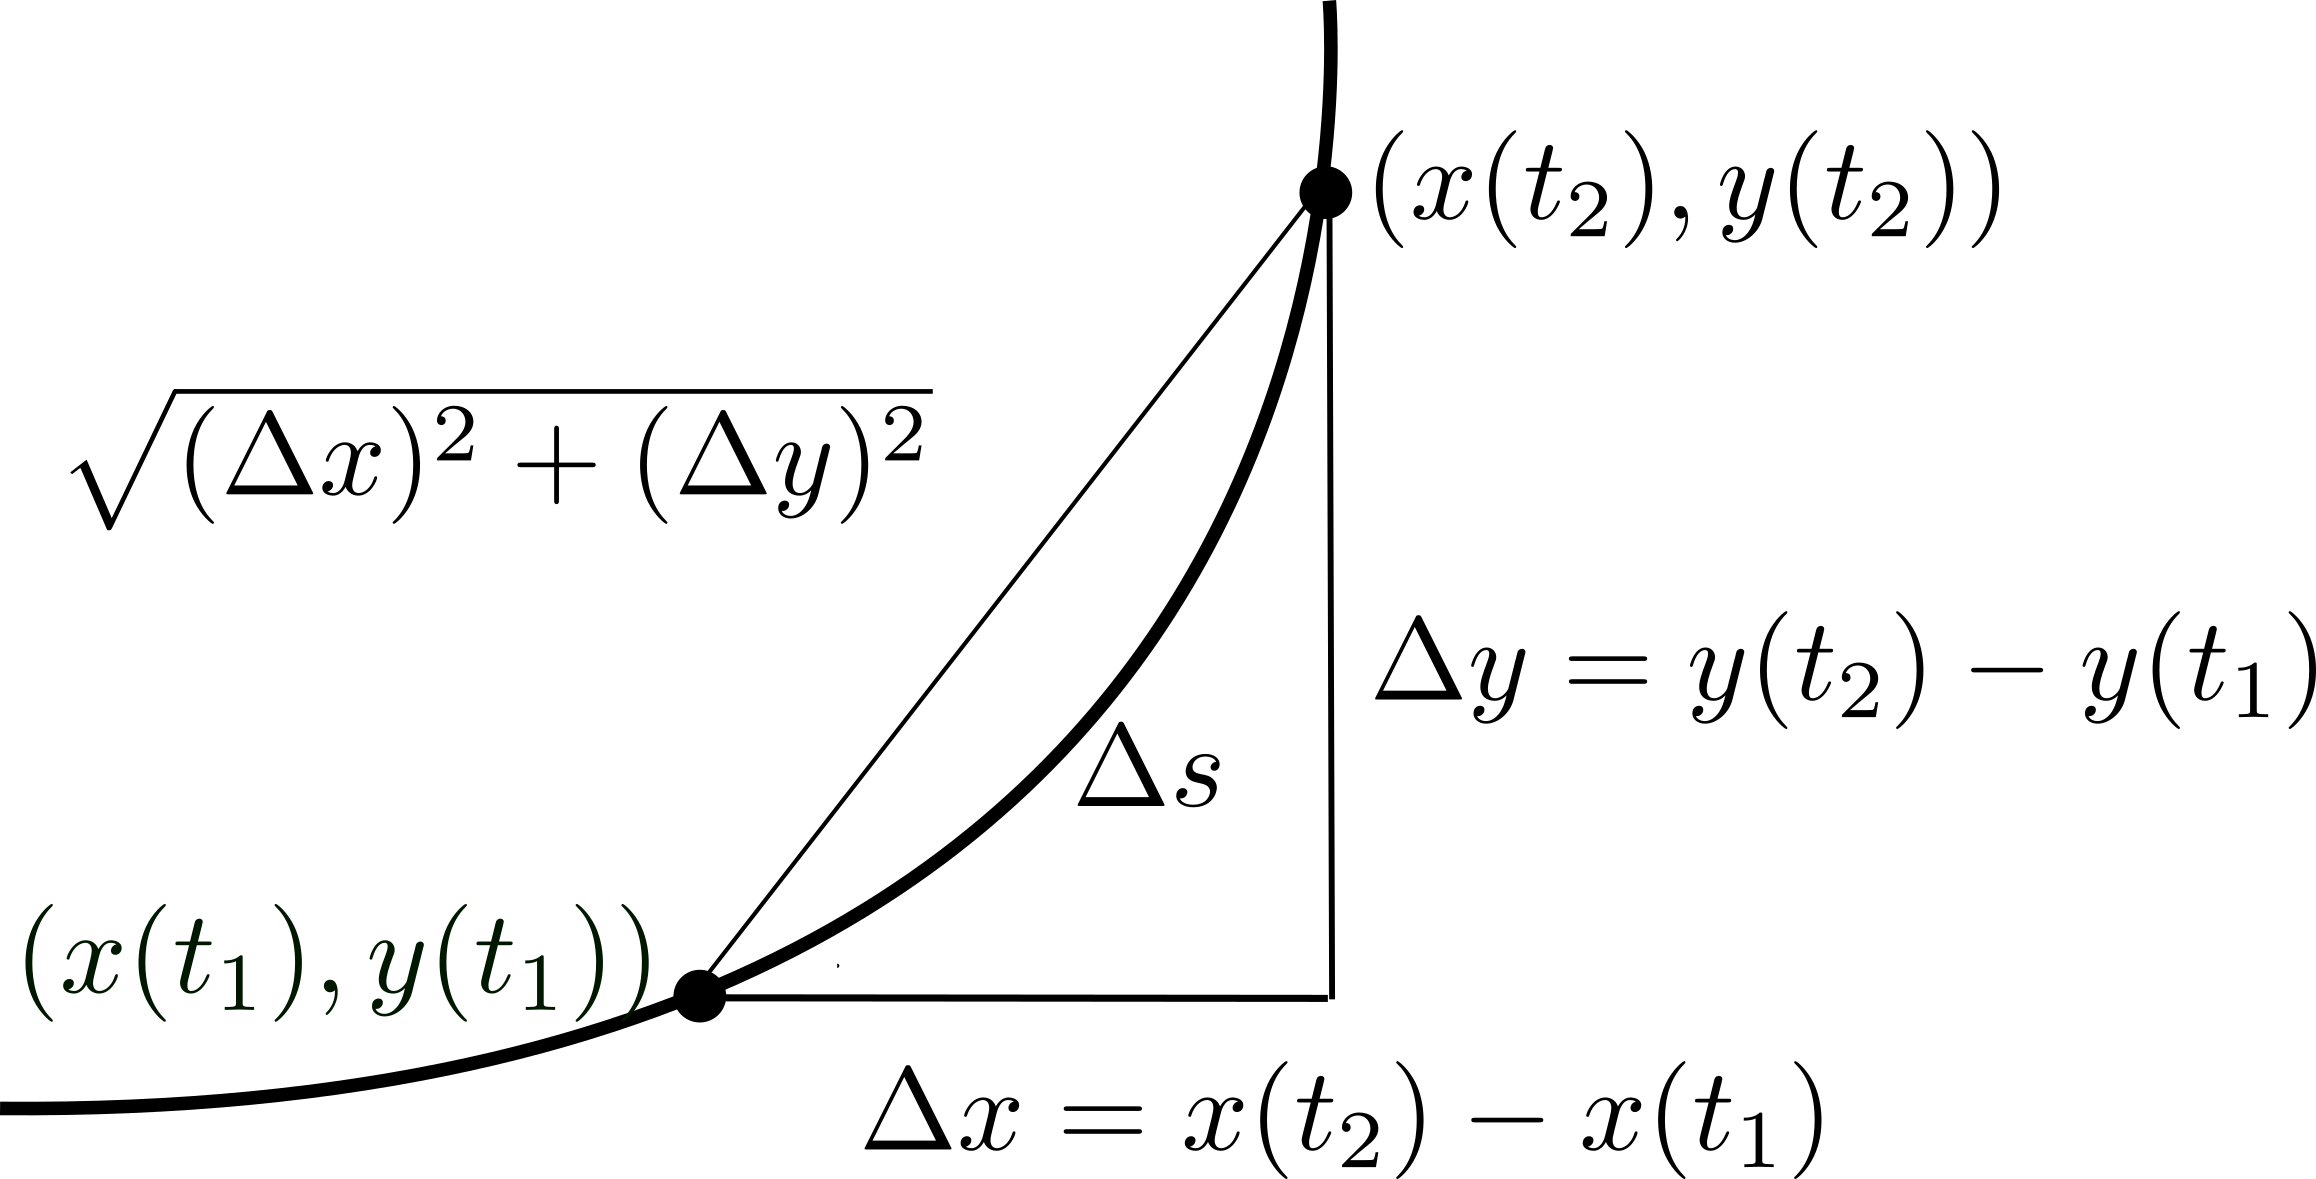
\includegraphics[width=100mm]{curve_length_2.png}
	\end{minipage}
	\begin{itemize}
		\item When $\Delta t = t_2 - t_1$ is small
		\item $\Delta s \approx	\sqrt{\left(\Delta x\right)^2 + \left(\Delta y\right)^2} $
		\item $\frac{\Delta s}{\Delta t} \approx	\sqrt{\left(\frac{\Delta x}{\Delta t}\right)^2 + \left(\frac{\Delta y}{\Delta t}\right)^2 } $
	\end{itemize}
\end{tcolorbox}

Now we're going to look at how long a curve is. 

We are can approximate the curve by a polygon by chopping up the curve into small pieces and summing the length the polygon. The length of the Polygon will converge to the curve length as we make the curve segments smaller and smaller.

Let's look at one small segment.  Choose 2 values of $t$,  $t_1$ and $t_2$, which are close. 

Then we can approximate the arc length $\Delta s$ between,  $t_1$ and $t_2$, by using Pythagoras’s theorem.

Dividing through by $\Delta t$ both sides we have approximate the rate change of the curve length by the rate of change of the $x$ and $y$ values or coordinates of the function.


\section{Length of a curve}
\begin{tcolorbox}
	\begin{itemize}
	\item As $\Delta t \to 0$
	\[
		\frac{ds}{dt} = \sqrt{\left( \frac{dx}{dt} \right)^2 + \left( \frac{dy}{dt}\right)^2}
	\]
	\item Integrate with respect to $t$ 
	\[
	s =\int_{a}^{b} \sqrt{x'(t)^2 + y'(t)^2}dt
	\]
	where $x'(t) = \frac{dx}{dt}$ and $y'(t) = \frac{dy}{dt}$
	\end{itemize}
	\begin{theorem}[Arc Length]
		The arc length between two points, $t = a$ and $t = b$, on the curve is given by
		$s =\int_{a}^{b} \sqrt{x'(t)^2 + y'(t)^2}dt$
	\end{theorem}	
\end{tcolorbox}

As we make the difference between $t_1$ and $t_2$ smaller and smaller i.e. we let $\Delta \to 0$ we can calculate the derivative of arc length with respect to the parameter $t$ as function of the first derivates of both $x(t)$ and $y(t)$ which is given here.

Now we can calculate the whole length of the curve by integrating with respect to parameter $t$. 

This gives us the to get the derivation of the arc length in terms of the first derivatives of both $x$ and $y$. 

Note that for my talk I will use the shorthand $x'(t)$ and $y'(t)$ to be the first derivatives of $x(t)$ and $y(t)$ respectively.

\section{Deriving formula for curvature}
\begin{tcolorbox}
	\begin{minipage}{\linewidth}
	\centering
		\centering
		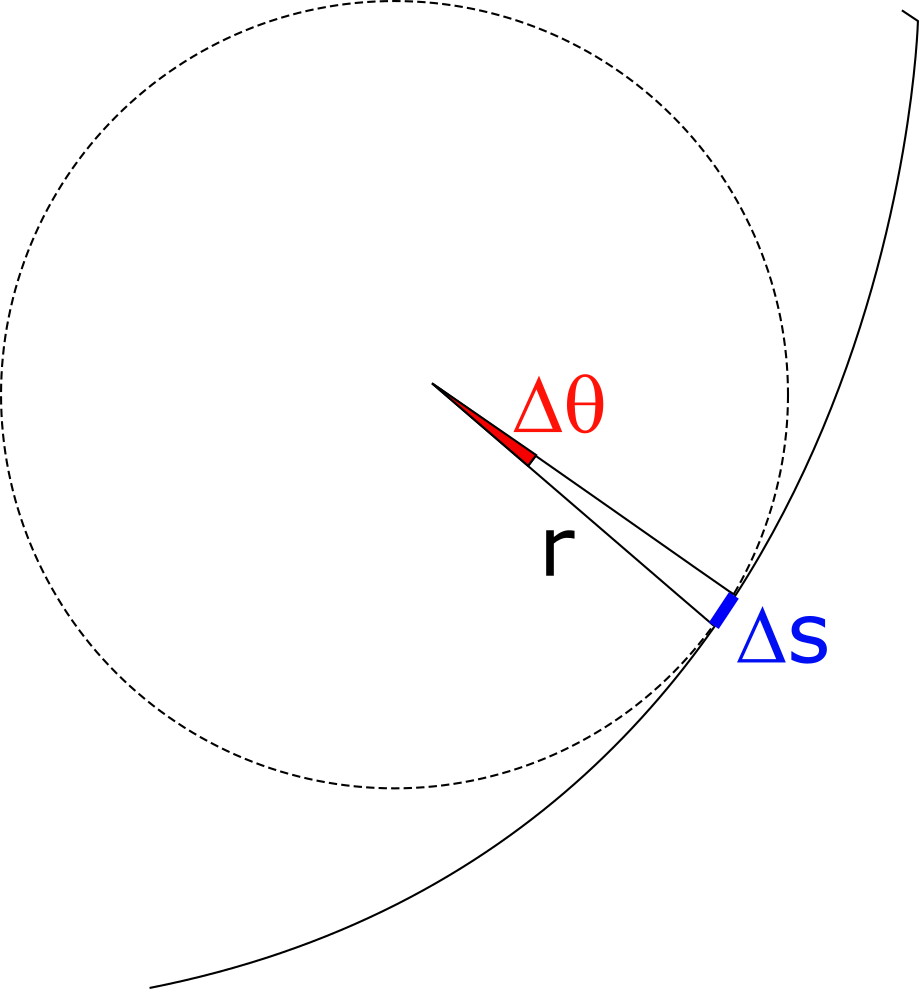
\includegraphics[width=50mm, scale=0.4]{curvature_illustration.png}
	\end{minipage}
	\begin{itemize}
		\item Firstly curvature is 1/radius of the osculating circle.
		\item Or the rate of change of the angle the tangent makes with the x axis with respect to arc length.
		\item $ds=rd\theta$ $\implies$ $\frac{1}{r}=\frac{d\theta}{ds}$	
		\item From arc length 
		\begin{equation} \label{eq:1}
			\frac{ds}{dt} = \sqrt{x'(t)^2+y'(t)^2} 
		\end{equation}
	\end{itemize}
\end{tcolorbox}

Now we move on to curvature. Curvature is a little be more tricky but the idea is straightforward.

Curvature is defined as the reciprocal of the radius of a circle which approximates the curve at a point. The approximating circle is called the osculating circle.

For the osculating circle the small circular segment or arc $\Delta s$ spanned by the small central angle $\Delta \theta$ must be equal to the arc length of the curve at that point. In which case $\Delta s = r \Delta \theta$.

We let $\Delta \theta \to 0$ so that in the limit $\frac{1}{r}=\frac{d\theta}{ds}$.

We calculate $\frac{d\theta}{ds}$ in two parts. First we calculate the rate of change of $s$ w.r.t. $t$, $\frac{d\theta}{ds}$ which we already know.

Second we calculate $\frac{d\theta}{dt}$

\section{Deriving formula for curvature}
\begin{tcolorbox}
	\begin{minipage}{\linewidth}
		\centering
		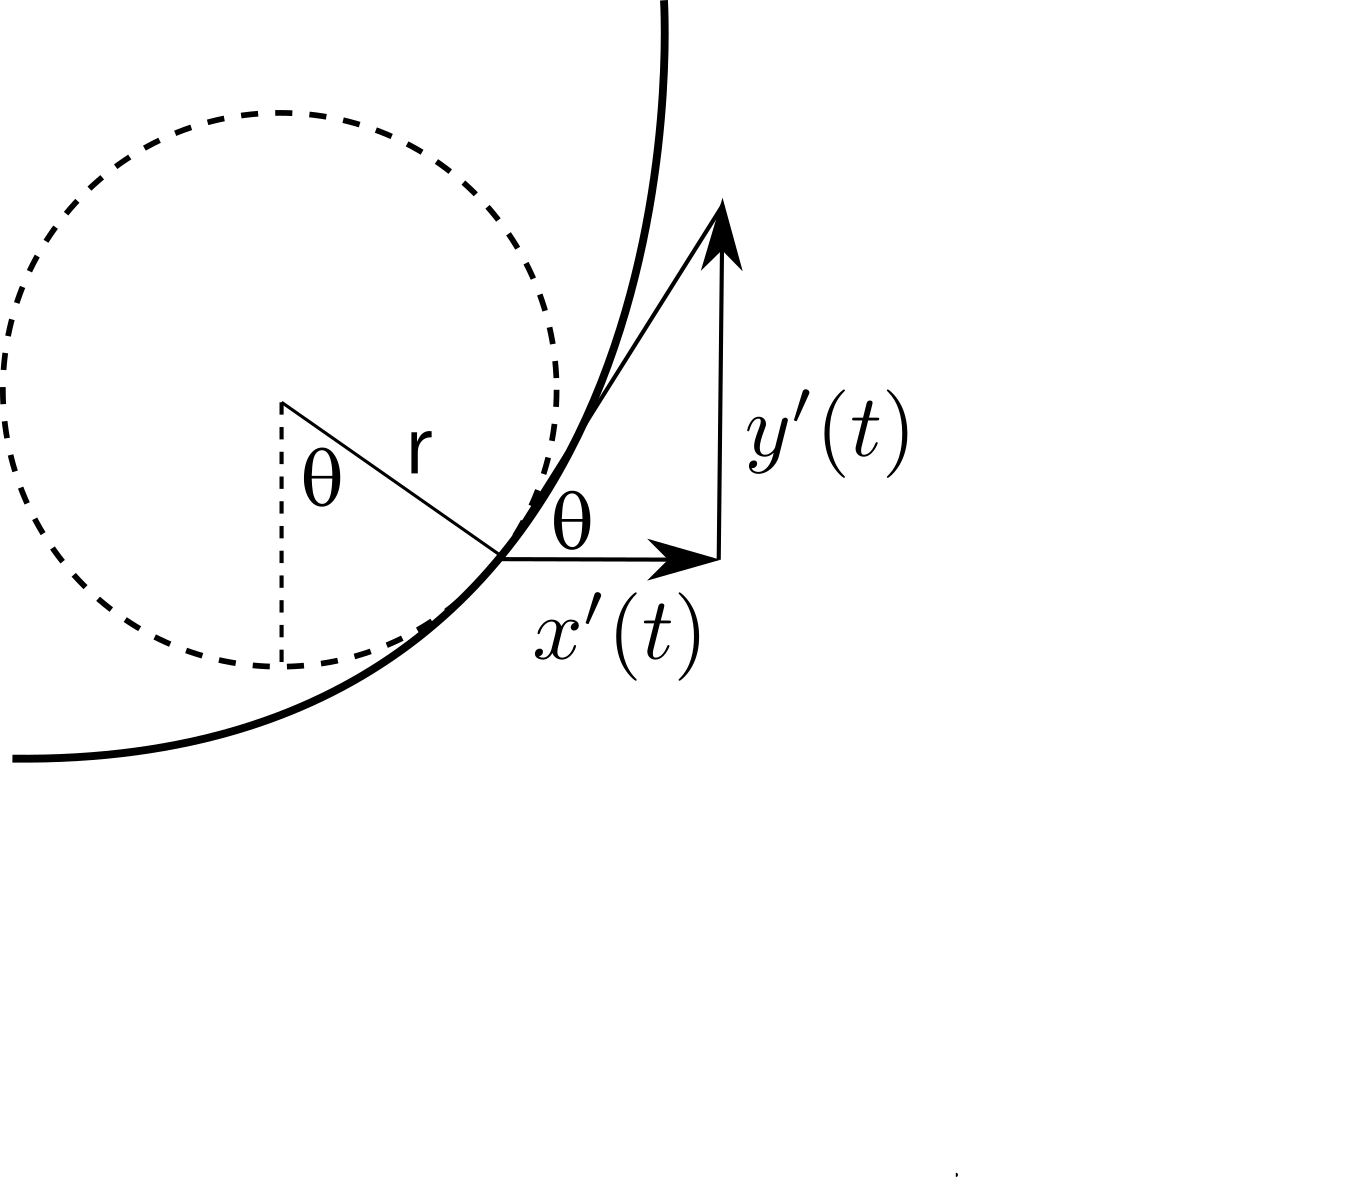
\includegraphics[width=75mm, scale=0.65]{curvature_illustration_2.png}
	\end{minipage}
	\begin{itemize}
		\item $\tan \theta = \frac{y'(t)}{x'(t)}$ 
		\item Differentiate w.r.t. $t$ gives $\sec ^2 \theta \frac{d\theta}{dt} = \frac{x'(t) y''(t) - y'(t) x''(t)}{x'(t)^2}$
		where $x''(t)=\frac{d^2 x}{dt^2}$ and $y''(t)=\frac{d^2 y}{dt^2}$
		\item $sec^2\theta = tan^2\theta +1 = \frac{{x'(t)^2+y'(t)^2}}{x'(t)^2}$ 
		\item Therefore
		\begin{equation} \label{eq:2}
			\frac{d\theta}{dt}=\frac{x'(t) y''(t) - y'(t) x''(t)}{x'(t)^2+y'(t)^2}
		\end{equation}
	\end{itemize}
\end{tcolorbox}

To calculate $\frac{d\theta}{dt}$ we notice that at the point where the circle touches the curve the slope of tangent to the curve and the circle must be the same.

The gradient of the tangent line is just the rate of change in the $y$ coordinate divided by the rate of change in $x$ coordinate.

Using the definition of $\tan$ we have that the angle $\theta$ must satisfy  $\tan \theta = \frac{y'(t)}{x'(t)}$.

Taking first derivatives w.r.t. $t$ we get on the left hand side $\sec ^2 \theta \frac{d\theta}{dt}$ and on the right had side $\frac{x'(t) y''(t) - y'(t) x''(t)}{x'(t)^2}$ using the quotient rule for derivatives.

Again using some trigonometric definitions we have that $sec^2\theta = tan^2\theta +1$ 

Finally collecting all the terms to the right hand side we have derived a formula for the rate of change of $\theta$ the central angle with respect to the parameter $t$ of the curve.

Again note that we are using the double dash-notation for the second derivates of $x$ and $y$.

\section{Deriving formula for curvature}
\begin{tcolorbox}
	\begin{itemize}
		\item Combining equations \ref{eq:1} and \ref{eq:2} gives us
		\begin{eqnarray*}
			\frac1r &=& \frac{d\theta}{ds} \\
					&=& \frac{d\theta/dt}{ds/dt}  \\
			        &=& \frac{x'(t) y''(t) - y'(t) x''(t)}{\left(x'(t)^2 + y'(t)^2 \right)^{3/2}}
		\end{eqnarray*}	
		\item Curvature, $\kappa = \frac1r$
	\end{itemize}
\end{tcolorbox}

Now we can put the two equations for the rate of change of the arc length and the rate of change of the central angle together.

Finally we note that the curvature is the reciprocal of the osculating circle.

\section{How curved is a curve?}
\begin{tcolorbox}
	\begin{theorem}[Curvature]
		The curvature of curve is $\kappa$ which is the reciprocal of the radius of the osculating circle given by
		\[
		\kappa=\frac{x'(t) y''(t) - y'(t) x''(t)}{\left( x'(t)^2 + y'(t)^2 \right)^{3/2}}
		\]
	\end{theorem}
	\begin{minipage}{\linewidth}
		\centering
		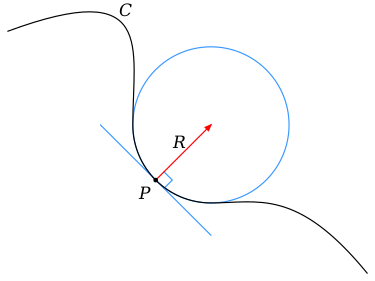
\includegraphics[width=75mm, scale=0.4]{Curvature_circle.png}
	\end{minipage}
\end{tcolorbox}

Thus we get our result for curvature. 

The smaller the radius the greater the curvature.

Conversely the greater the radius the smaller the curvature.

If both $x''(t)=0$ and $y''(t)=0$ then curve has no curvature - which is of course a straight line. For a straight line the osculating circle has infinite radius!

So for the curve to have curvature, we need at least one of $x''(t)$ and $y''(t)$ to be non-zero for some $t$.

Let's look at two simple examples to understand parametric curves, curvature and arc length.

\section{Curvature of a circle}
\begin{tcolorbox}
	\begin{itemize}	
	\item Circle: The parametric equations for a circle with radius $r$ are $x(t)=r \cos(t)$ and $y(t)= r \sin(t)$. 
	\item The arc length is 
	\[	
	s = \int_{0}^{2 \pi} \sqrt{r^2 \sin^2 t + r^2 \cos^2 t}dt = \left[r \right]_{0}^{2 \pi} = 2 \pi r
	\]
	\item Using the same parametrisations we can work out the curvature
	\[
	\kappa = \frac{r^2 \sin^2 t + r^2 \cos^2 t}{\left(r^2 \sin^2 t + r^2 \cos^2 t \right) ^ \frac{3}{2}} = \frac{1}{r}
	\]
	\end{itemize}
\end{tcolorbox}

Our first simple example is circle centred on $(0,0)$ which we know what the arc length and curvature should be.

For a circle the arc length should be $2 \pi r$ and the curvature should be $\frac{1}{r}$ since the circle its own osculating circle.

First, we need parametrise the circle. This is really easy. We just use the angle as our parameter $t$. Therefore $x(t)=r \cos(t)$ and $y(t)= r \sin(t)$.

If we calculate the first and second derivatives for $x$ and $y$ we get exactly what we expect. Phew!

\section{Parabola curve length}
\begin{tcolorbox}
	\begin{itemize}			
		\item Parabola: For parabola $y=x^2$ the parametric equations are $x(t)=t$ and $y(t)=t^2$. The arc length between 0 and 1 is 
		\begin{eqnarray*}
			s &=& \int_{0}^{1} \sqrt{1+4t^2}dt \\ &=& \left[\frac{1}{2} t\sqrt{1+ 4 t^2} +\frac{1}{4} \ln \left(2 t+\sqrt{1+ 4 t^2} \right) \right]_{0}^1 \\
			&\approx&	 1.48
		\end{eqnarray*}
	\begin{minipage}{\linewidth}
		\centering
		\includegraphics[width=50mm, scale=0.4]{Parabola_Arc_Length.png}
	\end{minipage}
	\end{itemize}
\end{tcolorbox}

Our second example is a parabola. The parameterisation for the parabola is straightforward we make our $x$-coordinate the parameter. 

In which case $x'(t)=1$ and $y'(t)=2 t$. Plugging this into the equation the arc lenght formula gives us an integral which we can evaluate in closed form.

The arc length between $0$ and $1$ is then $1.48$. You can compare that with the the length of the triangle with sides of length 1. Which would be $1.41$, thus we can see the "extra" length due curvature of the parabola compared to the straight line.

\section{Parabola curvature}
\begin{tcolorbox}
	\begin{itemize}	
		\item Parabola: Recall $x(t)=t$ and $y(t)=t^2$. 
		\[
		\kappa = \frac{2}{\left(1 + 4t^2 \right) ^ \frac{3}{2}}
		\]
		\begin{minipage}{\linewidth}
			\centering
			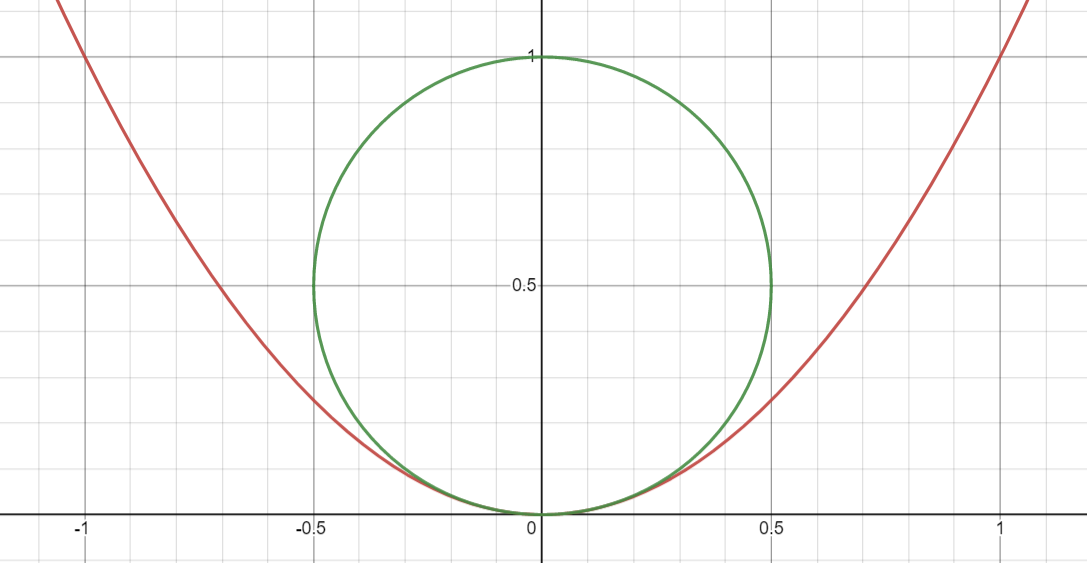
\includegraphics[width=50mm, scale=0.4]{Parabola.png}
		\end{minipage}
	\end{itemize}
\end{tcolorbox}
The second derivatives are $x''(t)=0$ and $y''(t)=2$. Plugging this into the formula for curvature we get $\kappa = \frac{2}{\left(1 + 4t^2 \right) ^ \frac{3}{2}}$.

We see that the parabola has the largest curvature when $t=0$ i.e. at the vertex of the parabola. Again as we would expect that is where the parabola is most ``bendy". In this case the curvature is 2.

At $t$ get bigger however the curvature falls and become more ``straight".

Question: From this example we see that we have two equations in terms of $t$. Do we really need $t$ or could we get rid of $t$? For example we could try to solve for $t$ in terms of $\kappa$ or $s$ and plug into the function $x$ and $y$? Wouldn't that be more  natural? That's what we're going to do next \dots.

\section{Relating curve length to curvature}
\begin{tcolorbox}
	Let's try the following parametrisation for $x$ and $y$
	\begin{eqnarray*}
		x(t) &=& \int_{0}^{t} \cos f(u) du \\
		y(t) &=& \int_{0}^{t} \sin f(u) du
	\end{eqnarray*}
	This gives us
	\begin{eqnarray*}
		x' = x'(t) = \cos f(t) &\mbox{ and }& x''=-f'(t) \sin f(t) \\
		y' = y'(t) = \sin f(t) &\mbox{ and }& y''=f'(t) \cos f(t)
	\end{eqnarray*}
\end{tcolorbox}

To directly relate the curve length to curvature we use the following parametrization of $x$ and $y$. 

Why does this turn out to be a ``good'' parametrization? Let's use the formulas for curvature, but first we need to get the first and second derivatives.

\section{Relating curve length to curvature}
\begin{tcolorbox}
	The slope, arc length and curvature now are:
	\begin{eqnarray*}
	\frac{dy}{dx} &=& \frac{\sin f(t)}{\cos f(t)} = \tan f(t) \\
 	s &=& \int_0^t \sqrt{\cos^2 f(u) + \sin^2 f(u)} du = t \\
 	\kappa &=& \frac{f'(t) \cos^2 f(t) + f'(t) \sin^2 f(t)}{\cos^2 f(t) + \sin^2 f(t)} = f'(t)
 \end{eqnarray*}
	\begin{enumerate}
		\item We can replace the variable $t$ by arc length $s$.
		\item And curvature at point $t$ is $f'(t)$. 
	\end{enumerate}
\end{tcolorbox}

We saw from the derivation of the curvature that the slope of the curve or the tangent at any point is just $\frac{y'(t)}{x'(t)}$ which we can relate to the angle for the tangent to the $x$-axis.

More importantly we have that $s=t$. Thus we have gotten rid of the nuisance parameter $t$ and replaced it with a natural parameter $s$ the curve length.

And curvature is now a function of arc length $s$! 

So we need to do define the curvature function $\kappa$ in terms of arc length $s$.

What does this mean for our curve function?

\section{Define the curve by curve length and curvature}
\begin{tcolorbox}
	 This all implies
	 \[
	 f(u) = \int_{0}^{u} \kappa(t) dt
	 \]
	Thus the equations for the curve become
	\begin{eqnarray*}
	x = x(s) &=& \int_{0}^{s} \cos \left( \int_0^u \kappa(t) dt \right) du \\
	y = y(s) &=& \int_{0}^{s} \sin \left( \int_0^u \kappa(t) dt \right) du
	\end{eqnarray*}
	Hence the curve is defined by arc length and curvature alone!
\end{tcolorbox}

So if we define our curvature function $\kappa$ as a function of curve length $s$ we can replace the integrand $f(u)$ before by an integral of curvature $\int_{0}^{u} \kappa(t) dt$. This is a measure of the total curvature we have see along the curve.

And finally we have a curve defined in terms of the curvature function and the arc length alone and we have a natural parameter $s$.

This is a special case of a advanced theorem in differential geometry called the ``fundamental theorem of plane curves'' which states that curvature in $\mathbb{R}^2$ defines the curve up to a translation and rotation (which are the constants of integration).


\section{A very simple example}
\begin{tcolorbox}
	Suppose the curvature $\kappa$ constant and equal to 1. 
	
	Then 
	$ \int_0^u \kappa(t) dt = u $ and
	\begin{eqnarray*}
		x = x(s) &=& \int_{0}^{s} \cos u du = \sin s\\
		y = y(s) &=& \int_{0}^{s} \sin u du = - \cos s + 1
	\end{eqnarray*}
	which is the parametric curve for a circle with centre $(0, 1)$ and radius $1$ - as expected.
\end{tcolorbox}

We know that the curvature is constant for a circle. Do we get back the equation for a circle if we use this curvature function? The answer is yes?


\section{The Euler spiral}
\begin{tcolorbox}
	Euler defined his curve as one where the curvature is proportional to arc length.
	
	\begin{center}
		\boxed{\kappa(s) = s}
	\end{center}
	Then 
	$ \int_0^u \kappa(t) dt = \frac{u^2}{2} $ and
	\begin{eqnarray*}
		x = x(s) &=& \int_{0}^{s} \cos \frac{u^2}{2} du\\
		y = y(s) &=& \int_{0}^{s} \sin \frac{u^2}{2} du
	\end{eqnarray*}
	But since these integrals can't be solved analytically how were they calculated?
\end{tcolorbox}

A more interesting example is when we let the curvature function be proportional to the curve length. To keep things simple let's set the constant of proportionality to 1.

In this case we have that the integrand for $x$ and $y$ becomes $\cos \frac{u^2}{2}$ and $\sin \frac{u^2}{2}$. And we get two integrals for the $x$ and $y$ coordinates which have not analytic solutions. 

This is exactly the formulation derived by Euler in 1744. But why did Euler come up with this formulation in the first place and how did he try to solve these integrals?


\section{Solving the integrals: Euler}
\begin{tcolorbox}
	\begin{itemize}
		\item In 1744 Euler derived these integrals.
		
		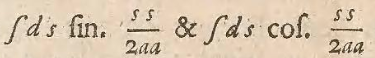
\includegraphics[width=50mm, scale=0.5]{euler_scripture_1.png}	
		\item He derived a series expansion which is still a viable method for small $s$.	
		
		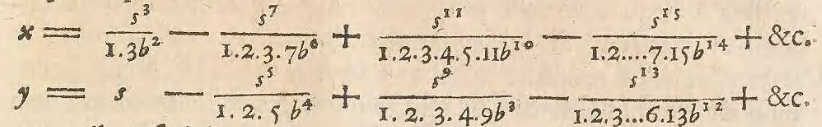
\includegraphics[width=100mm, scale=0.7]{euler_scripture.png}
		\item In 1781 he proved the integrals for limits between 0 and $\infty$ are equal to  $\frac{a \sqrt{\pi}}{2}$ where $a=1$ for the Euler spiral.
	\end{itemize}
\end{tcolorbox}

In the first bullet we see the derivations for $y$ and $x$ from his 1744 book where he proved the result for the cantilever problem. What I found really interesting is that I could read his results even though they are almost 300 years old.

In the second bullet we see his attempts to solve the integrals for small values of s which are still a good way of evaluation the integral for small $s$.

Amazingly he was able to solve exactly the limiting case where $s \to \infty$ in 1781. 


\section{Solving the integrals: Fresnel}
\begin{tcolorbox}
	\begin{itemize}
		\item Fresnel rediscovered these integrals when investigating the diffraction of light through a slit. He showed that the light intensity (under some assumptions) was 
		\[
		\left( \int_{0}^{s}\cos \left( \pi t^2 / 2 \right) dt \right) ^2 + 
		\left( \int_{0}^{s}\sin \left( \pi t^2 / 2 \right) dt \right) ^2
		\] 
		\item These integrals are the same as the ones Euler derived (up to a factor of $\pi$).
		\item Integrals are called the \emph{Fresnel integrals}.
		\item Fresnel calculated them for values of $s$ between 0.1 and 5.1.
	\end{itemize}
\end{tcolorbox}

In 1818 Augustin Fresnel rediscovered these integrals when he investigated the diffraction of light through a slit. 

In 1874 Alfred Cornu calculated values and plotted the Euler spiral accurately. Hence the Euler spiral is also known as a Cornu spiral.


\section{Solving the integrals: using Python}
\begin{tcolorbox}
	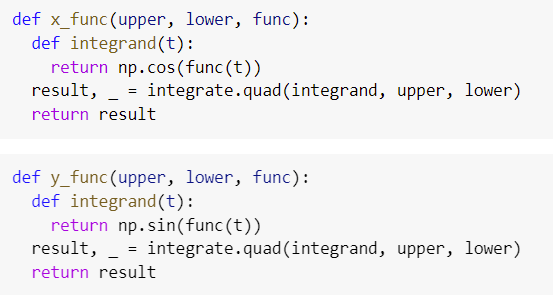
\includegraphics[width=50mm, scale=0.5]{code_1.png}	
			
	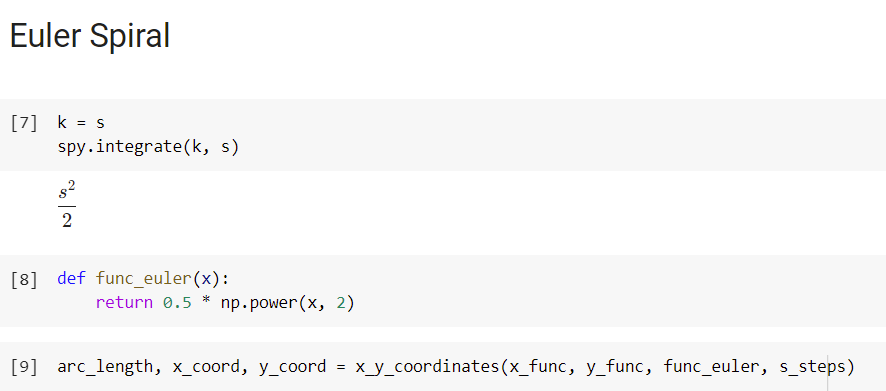
\includegraphics[width=50mm, scale=0.5]{code_2.png}
	
	Nowadays computers and numerical methods are used to evaluate these integrals.
\end{tcolorbox}

To solve these integrals I used a numerical integration technique available in the Python, which  are very fast and easy to use. 

\section{The Euler spiral - $x$ $y$ Coordinates}
\begin{tcolorbox}
	\begin{minipage}{\linewidth}
		\captionof{figure}{Fresnel integrals with arguments $\frac{u^2}{2}$}
		\centering
		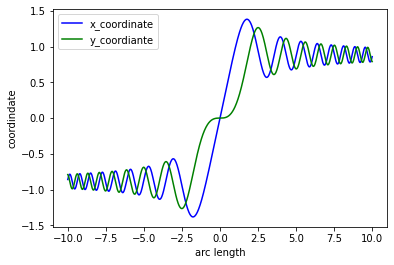
\includegraphics[width=70mm, scale=0.5]{euler_x_vs_y.png}
	\end{minipage}
	As expected these converge to $\pm \frac{\sqrt{\pi}}{2} \approx 0.8862$.
\end{tcolorbox}

Here I show the $x$ and the $y$ coordinate i.e. the Fresnel integrals.

We can see the sinusoidal curve as the arc length increases.

The oscillations dampening as the arc length increases. 

We also see that they seem to converge to the limits calculated by Euler: $\pm \frac{\sqrt{\pi}}{2}$. 

\section{The Euler Spiral}
\begin{tcolorbox}
	\begin{minipage}{\linewidth}
		\captionof{figure}{The Euler spiral aka Cornu spiral}
		\centering
		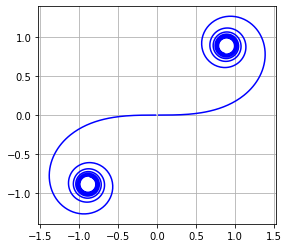
\includegraphics[width=70mm, scale=0.5]{euler_spiral.png}
	\end{minipage}
\end{tcolorbox}

When we plot the $x$ and $y$ coordinates against each other we see a distinctive spiral shape. 

Starting at (0,0) the further we go along the curve the more curved it gets. Indeed it gets so curved that starts bending back in itself in an every tighter spiral!

Note that when $s<0$ the curvature is negative i.e. the curve is turning \emph{clockwise} or \emph{to the right} in that region as $s$ increases. 

In contrast when $s>0$ the curvature is positive, i.e. the curve is turning \emph{counter-clockwise} or \emph{to the left} in that region as $s$ increases.


\section{Euler's first drawing}
\begin{tcolorbox}
	\begin{minipage}{\textwidth}
		\centering
		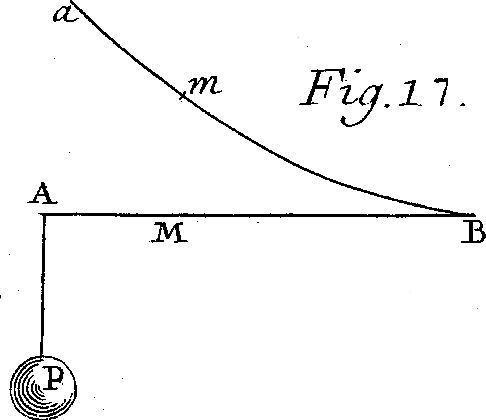
\includegraphics[width=.5\linewidth]{Euler_first_drawing.png}
		\captionof{figure}{Euler's first drawing from a 1744 publication. P refers to a weight.}
		\label{fig:test1}
	\end{minipage}
	\begin{minipage}{\textwidth}
		\centering
		\includegraphics[width=0.5\linewidth]{Euler second drawing.png}
		\captionof{figure}{Euler's drawing of full spiral in 1781 after solving integrals to $\infty$}
		\label{fig:test2}
	\end{minipage}

\end{tcolorbox}

In these pictures we see Euler's first drawings of part of this curve. 

The figure on the left shows his solution to the ``Cantilever problem''.

The ``Cantilever Problem'' first posed in 1694 James Bernoulli. He asked: What shape must a pre-curved thin beam fixed at one end have in order to be horizontal and straight when a weight is added to the non fixed end? 

Bernoulli claimed the curvature increased along the beam and was proportional to the distance along the beam. But he never provided a proof.

It was not until 1744 that Euler proved the result and attempted his first calculations.

The curve $a-B$ is the pre-curved beam before the weight has been put on one end. Notice how the curve starts flat and gets more curved as it reaches the fixed end.

Euler's showed that when the curve is horizontal when the mass $P$ is attached to the end $A$.

The right hand chart shows the convergence of the spiral to the limit of the integral.

\section{Other fun curves: even powers of $s$}
\begin{tcolorbox}
	\begin{minipage}{\linewidth}
	\captionof{figure}{$\kappa(s) = s^2$}
	\centering
	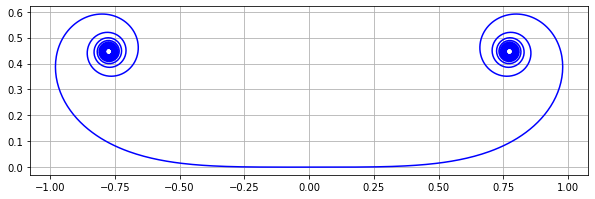
\includegraphics[width=85mm, scale=0.5]{chaise_longue.png}
\end{minipage}
\end{tcolorbox}

In this case the curvature is positive for all $s$, even the region $s<0$ so the curve is bending to the left or counter clockwise for all values of $s$, as $s$ increases.

\section{More fun curves: mix in a bit of a circle}
\begin{tcolorbox}
	\begin{minipage}{\linewidth}
		\captionof{figure}{$\kappa(s) = s ^ 2 -2.19$}
		\centering
		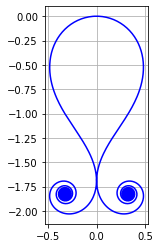
\includegraphics[width=35mm, scale=0.2]{s_squared_minus_219.png}
	\end{minipage}
\end{tcolorbox}

As we saw before a constant curvature is a circle. By subtracting a negative number from the previous curvature function we are pulling the sides, of the previous plot, down around circle until the two sides touch.

\section{More fun curves: polynomials}
\begin{tcolorbox}
	\begin{minipage}{\linewidth}
		\captionof{figure}{$\kappa(s) = 5 s ^ 4 - 18 s ^ 2 + 5$}
		\centering
		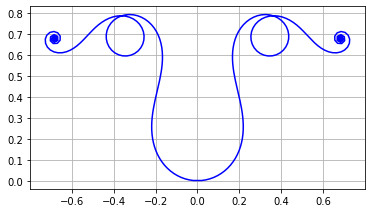
\includegraphics[width=70mm, scale=0.5]{five_s^4.png}
	\end{minipage}
\end{tcolorbox}

By adding polynomials terms of different orders we get loops of varying sizes as the different powers impact the curvature as varying rates.

For very small values of $s$ the constant term $5$ dominates which we know is a circle.

For slight larger values of $s$ of (approximately $s<\sqrt{18/5}$) the (negative) quadratic term dominates the curvature

For large values of $s$ the (positive) quartic term dominates the curvature.


\section{More fun curves: trigonometric functions}
\begin{tcolorbox}
	\begin{minipage}{\linewidth}
		\captionof{figure}{$\kappa(s) = \cos(s) - s \sin(s)$}
		\centering
		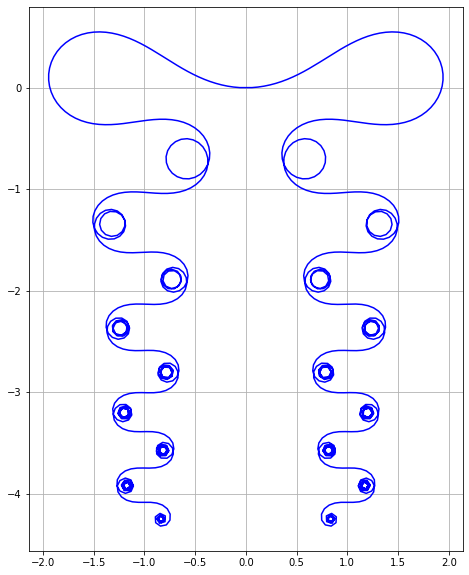
\includegraphics[width=50mm, scale=0.2]{elegant_madness.png}
	\end{minipage}
\end{tcolorbox}

Here we see curvature is impacted by sinusoidal behaviour where the amplitude of the curvature increases with arc length making the curvature oscillate very large positive and negative values.
	
\section{More fun curves: hyperbolic functions}
\begin{tcolorbox}
	\begin{minipage}{\linewidth}
	\captionof{figure}{$\kappa(s) = \sinh(s) - 5.19$}
	\centering
	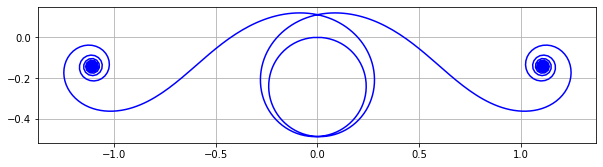
\includegraphics[width=100mm, scale=0.5]{sinh.png}
\end{minipage}
\end{tcolorbox}

In this case we look at the impact of exponential behaviour on curvature. 

For small values $s$ we have a circle with a radius of slightly larger that 0.2 ($1/5.19$).

But as $s$ increases the curvature increases exponentially.

\section{Application: Designing roads and railways}
\begin{tcolorbox}
	\begin{itemize}
		\item Euler's spiral was rediscovered by railway designers in the 19th century.
		\item Transition curves link straight sections of roads or railways.
		\item Designed to give passengers a smooth ride with no sudden changes in acceleration.
	\end{itemize}
	\begin{minipage}{\linewidth}
		\captionof{figure}{Cloverleaf motorway interchange}
		\centering
		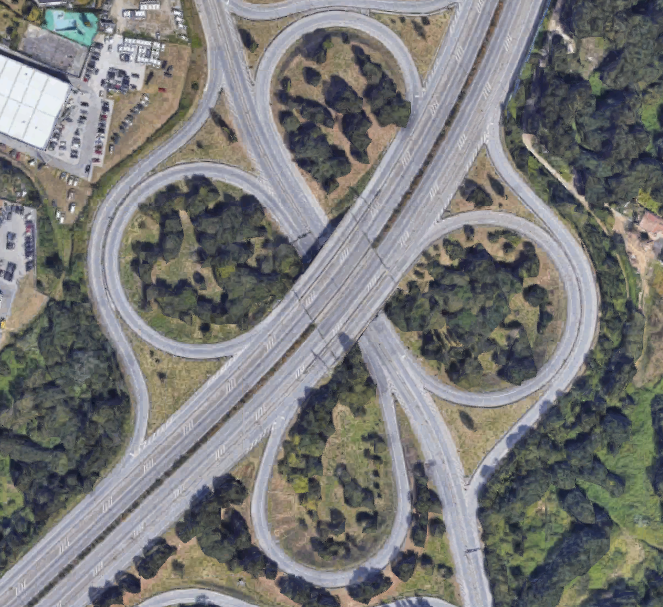
\includegraphics[width=40mm, scale=0.5]{cloverleaf_motorway.png}
	\end{minipage}
\end{tcolorbox}

Now we will look at an application that is all around us and is used by civil and railway engineers to design road and railway tracks.
 
As trains became faster in the 19th century, the Euler spiral was rediscovered by railway designers. Railway engineers discovered that a track shape with gradually varying curvature provided a smooth riding experience.

In 1899 railway engineer Arthur Talbot solved the problem mathematically and derived the same integrals as Fresnel. His solution was ``a curve whose degree-of-curve increases directly along the curve." He even derived a series expansion for the integrals almost identical to Euler's 1744 series that we saw earlier.

These curves are called transition curves and are used to link straight sections of road and railways.

Look at the bottom loop of this "clover leaf interchange". You would turn through almost 240 degrees if you went round that loop. 

Knowing what we know now we see the curvature starts very gently and the curvature increases with the arc length - until we reach the apex. Then we see the curvature decreases with arc length.

Now we look at why that is a "good behaviour" for transition curve.


\section{Why transition curves are Euler spirals}
\begin{tcolorbox}
	\begin{itemize}
	\item Acceleration along a transition curve is
 	 \[
 	 a=s''(t) \vec{T}+\kappa s'(t)^2 \vec{N}
 	 \]
 	 where $\vec{T}$ is the unit tangent vector and $\vec{N}$ is the unit normal vector, $s(t)$ is the curve length, $s'(t) = \frac{ds}{dt}$ and $s''(t) = \frac{d^2 s}{dt^2}$.
 	 \item If the car/train is going round the curve at constant speed $s'(t)=constant$ and $s''(t)=0$.	
 	 \item The acceleration at constant speed depends on the curvature $\kappa$ and speed $s'(t)$ in the direction of the normal vector.
 	 \item For smooth ride curvature should increase with curve length.
	\end{itemize}
\end{tcolorbox}

The general formula for acceleration along a curve is given here. 

It's made up of two components. First, the \emph{linear} acceleration along the straight line given by the tangent. Which is just the rate of change of speed along the curve or the the second derivative of curve length with respect to time.

Second, we have the \emph{angular} acceleration which is in the direction perpendicular to the tangent line - i.e. in the direction of the normal vector. This acceleration depends of the curvature (or reciprocal of the the radius of the osculation circle) and the square of the speed along the curve.

For our example suppose we want to maintain constant speed along the curve.

We want to avoid being thrown around in a car or train. Therefore we want the curvature to increase with curve length.

\section{Case 1: Semicircular transition curves}
\begin{tcolorbox}
	A closed  track is made up of four segments.
	\begin{enumerate}
		\item A straight track of length 1km
		\item A semicircular track of length 1km. This has radius $1,000 / \pi m \approx 318.31m$
		\item A straight track of length 1km
		\item A semicircular track of length 1km.
	\end{enumerate}
	Let the vehicle go around the track at a constant speed of $60 km/h = 16 \frac{2}{3} m/s$.
\end{tcolorbox}

To show you how an transition curve can be designed from bits of Euler spirals assume we have a track which is 4km long and made up of two straight segments and to curve segments. 

In the first case the two curves segments are made up of two semi-circular tracks - as you might have had in your Scalextric set when you were younger!

And assume that we're going around the track at constant speed of 60 km/h.

\section{Case 1: Position and acceleration}
\begin{tcolorbox}
	\begin{minipage}{\linewidth}
		\captionof{figure}{Position and acceleration}
		\centering
		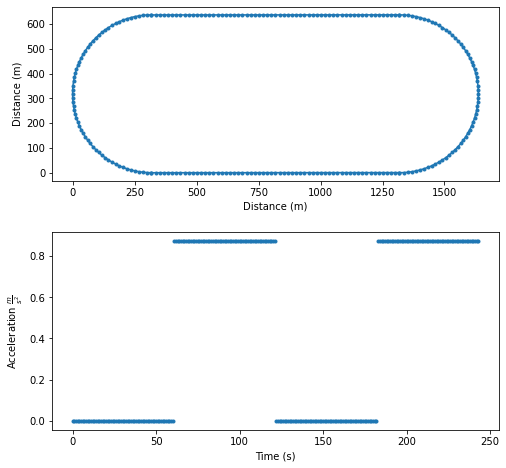
\includegraphics[width=70mm, scale=0.2]{circular_track.png}
	\end{minipage}
	Note: Acceleration is a step function. 
	
	As a passenger you feel the full centrifugal force ($F=mv^2/r$) pushing you outward the moment you entered the curve. 		
\end{tcolorbox}

Using the formula for speed and acceleration we can calculate our position every second. It would take 4 minutes to drive around the track.

Most importantly because we are going around at constant speed the instant we entered the turn we would feel the full centrifugal force pushing you outward.

This is uncomfortable for the driver and passengers. 

\section{Case 2: Euler spiral transition curves}
\begin{tcolorbox}
	\begin{itemize}
		\item A closed track with same width and height. 
		\item Replace semicircles with two half Euler Spirals.
		\item Curvature is proportional to arc length: $\kappa(s) = \alpha s $ for some $\alpha$.
		\item Width and height of an Euler Spiral that turns through $\pi/2$ is 
		\begin{eqnarray*}
			width &=& \sqrt{\pi / \alpha} C(1) \\
			height &=& \sqrt{\pi /\alpha} S(1)
		\end{eqnarray*}
		where $S(u)$ and $C(u)$ are the standard Fresnel integrals.
	\end{itemize}
	\[
		\alpha = \frac{\pi S(1)^2}{r^2} \approx 5.95 \times 10 ^{-6}
	\]
\end{tcolorbox}

To make the ride smooth we are going the create a track which has the same width and height as before but the curved ends are going to be made up of two half Euler spirals.

We are going to make the curvature increase proportionally with the length of the curve until you have turned through 90 degrees or $\pi/2$ radians and reached the apex of the curves. At that point the curvature is going to fall linearly until you leave the curve and have turned through 180 degrees of $\pi$ radians.

To calculate the constant of proportionality for the curvature, what I call $\alpha$, we need to make sure that the ``height'' of Euler spiral is equal to the radius of the circles we had before.

While I don't have time to discuss, one of the neat things about the Fresnel integral is that the integrands are scaled by $\pi/2$. Since we want to have turned through $\pi/2$ at the apex of the curve all we need to substitute $1$ into the Fresnel integral. Then all we need to do is scale the result to match the width with the radius. 


\section{Case 2: Euler spiral transition curves}
\begin{tcolorbox}
	\begin{minipage}{\linewidth}
		\captionof{figure}{Position and acceleration}
		\centering
		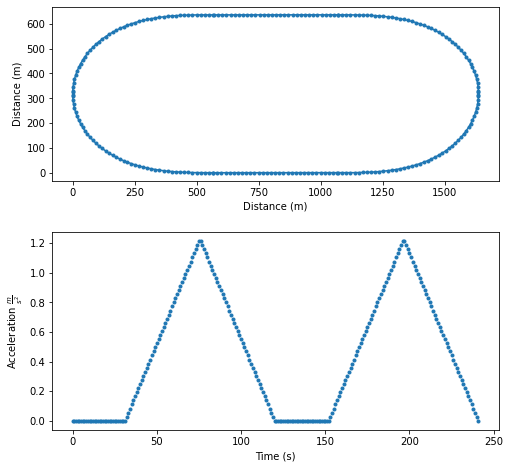
\includegraphics[width=70mm, scale=0.2]{euler_track.png}
	\end{minipage}
	Note: Acceleration increases linearly as we move through the curve.		
	The maximum acceleration at the apex is greater than with the semicircular track but the ride is now more comfortable.
\end{tcolorbox}

Here we see the track with transition curves based on Euler spirals. 

Again we look at position, and acceleration at 1 second intervals. 

Looking at the acceleration we see that acceleration increases linearly from the moment we enter the curve reaching a maximum at the apex of the curve. At the apex we feel more angular acceleration than in the circular track case. This is because the radius of the osculating circle at the apex is smaller than the radius of the semicircle.

However the ride will much smoother for the driver and the passengers.

As an aside you will also have noticed that the straight sections of the track are shorter since we have to start turning much earlier in the bend - the straight sections are only 504m long compare to 1,000m in the previous example.

\section{Thanks for listing}
\begin{tcolorbox}
	\centering
	Thanks for listening!
\end{tcolorbox}

That is it for my talk. I hope you've enjoyed this introduction to curvature, arc length and the genius of Euler again.

One final thought: so next time you turn off the motorway, you can thank Euler for not feeling ill and getting thrown around in your car - unless you're a racing driver but that's another story!

\end{document}
